\documentclass[a4paper]{report}
\usepackage[english]{babel}
\usepackage{amsfonts}
\usepackage{amsmath} % Equation numbering
\usepackage[square,sort,comma,numbers]{natbib}

\usepackage{graphicx} % Figures
\usepackage{grffile} % For recognising the png-extension
\usepackage{float} % For floating figures

\usepackage{changes} % For track changed extensions
\usepackage{todonotes}

\usepackage{dsfont} % For indicator function

\usepackage{hyperref}
\bibliographystyle{plainnat}

% For example environment
\usepackage{amsthm}
\theoremstyle{definition}
\newtheorem{example}{Example}[section]

% For theorem environment
\newtheorem{theorem}{Theorem}

\begin{document}
\chapter{Simulating a Markov Modulated Fluid Model}
From a generator matrix, a fluid jump matrix and a vector of fluid rates, the lifetime of a Markov Modulated Fluid Model is simulated in Matlab.
For three different states with fluid rates $1$, $2$ and $3$ respectively and transition intensities given by generator matrix
\begin{equation}
G=\begin{bmatrix}
-3& 1& 2\\ 1& -2& 1\\ 0&1&-1
\end{bmatrix}.
\end{equation}
A jump matrix with one jump is chosen
\begin{equation}
G=\begin{bmatrix}
0& 0& 5\\ 0& 0& 0\\ 0&0&0
\end{bmatrix}.
\end{equation}
We've simulated some samples with and without jumps, this results in the following hazard rates:
\begin{figure}[H]
\centering
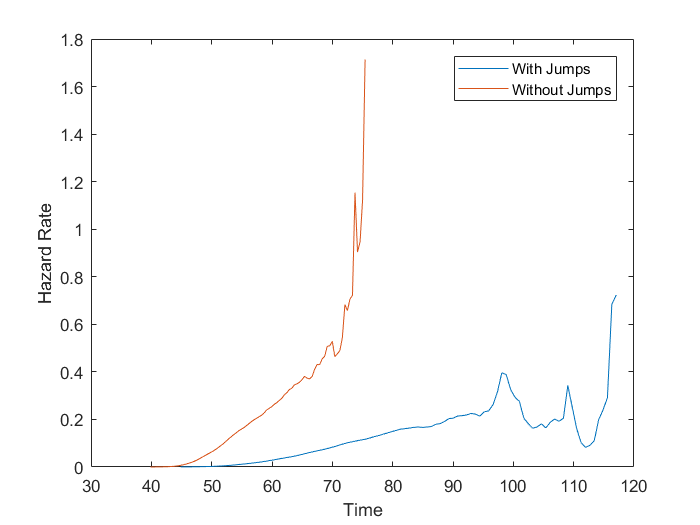
\includegraphics[width=\textwidth]{Plots/MmfmHazards.png}
\caption{The hazard rates of the simulated data.}
\end{figure}
As you can see, jumps increase the lifetime and make the hazard function less increasing.
\end{document}